In this section, we evaluate the performance of the proposed framework. Our
prototype of the framework had been implemented in the Go programming language
\cite{go}. The prototype is divided into multiple independent packages, and the
corresponding source codes are available online \cite{sources}. The source code
of the experimental setup below along with the input data are also available at
\cite{sources}. The experiments are conducted on a \abbr{GNU}/Linux machine
equipped with 16 processors Intel Xeon E5520 2.27~\abbr{GH}z and 24~\abbr{GB} of
\abbr{RAM}.

Each problem that we consider is structured as follow. A platform $\procs$ with
$\np$ processing elements and an application $\tasks$ with $\nt$ tasks are
generated randomly by the \abbr{TGFF} tool \cite{dick1998}. The tool generates
$\np$ tables and a directed acyclic graph with $\nt$ nodes. Each table
corresponds to a processing element, and it describes certain properties of the
tasks when they are mapped to that particular processing element. Namely, each
table assigns two numbers to each task: a reference execution time, chosen
uniformly between 10 and 50~ms, and a power consumption, chosen uniformly
between 5 and 15~W. The graph captures data dependencies between the tasks. The
application is scheduled using a list scheduler \cite{adam1974}. The mapping of
the application is fixed and obtained by scheduling the tasks based on their
reference execution times and assigning them to the earliest available
processing elements (a shared ready list).

The construction of thermal \abbr{RC} circuits needed for temperature analysis
is delegated to the HotSpot tool \cite{skadron2004}. The floorplan of each
platform is a regular grid wherein each processing element occupies $2 \times
2~\text{mm}^2$ on the die. The output of the tool is essentially a pair of a
thermal capacitance matrix $\mC$ and a thermal conductance $\mG$ matrix used in
\eref{thermal-system}. The leakage modeling is based on a linear approximation
\cite{yang2013, ukhov2012, liu2007}.

\begin{figure}[t]
  \centering
  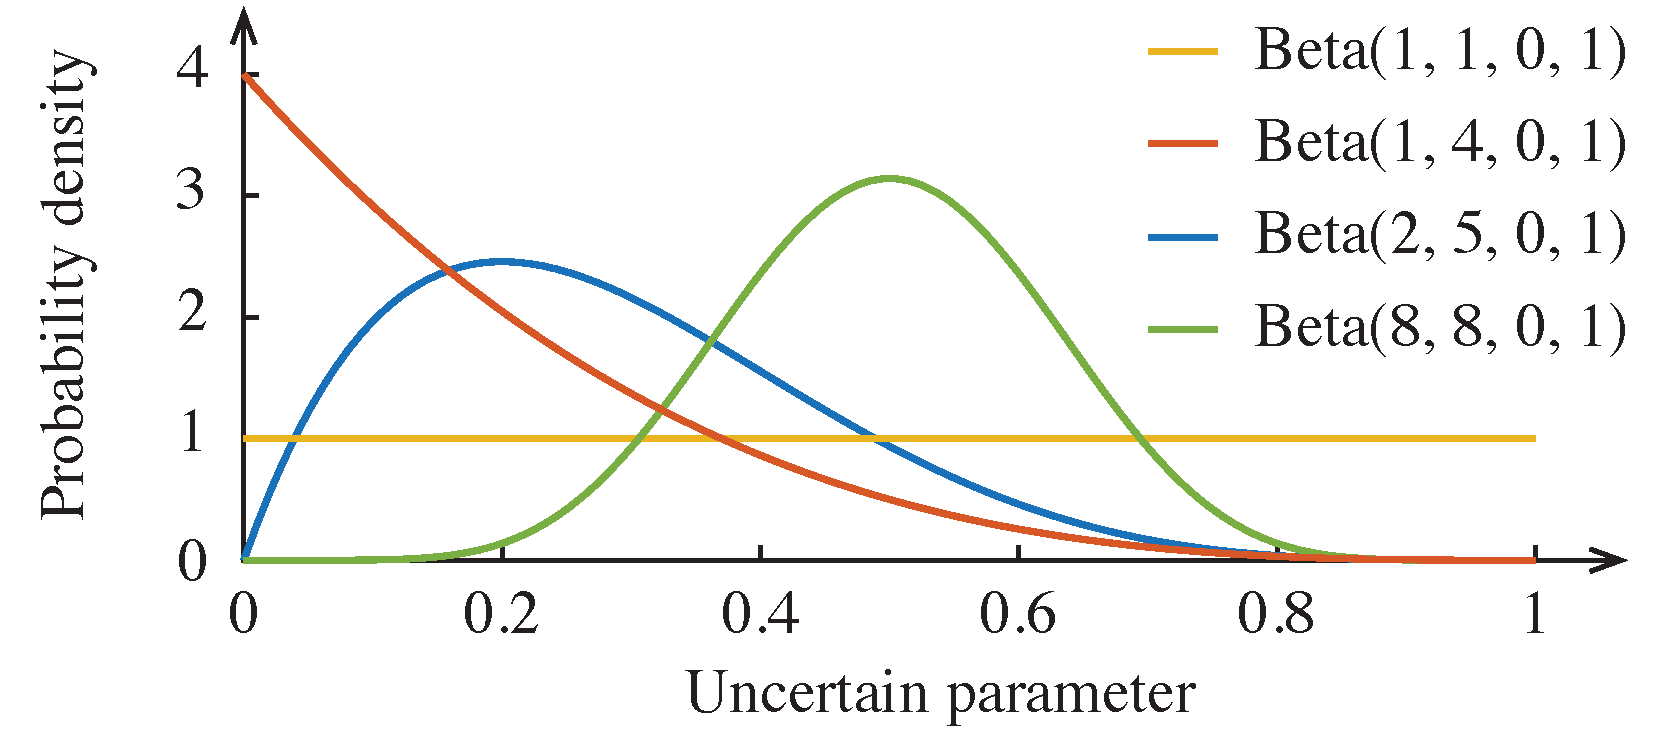
\includegraphics[width=1.0\columnwidth]{include/assets/figures/distribution.pdf}
  \caption{An illustration of the family of beta distributions.}
  \flab{distribution}
\end{figure}

The uncertain parameters $\vu$ are the execution times of the tasks; all other
parameters are deterministic. Targeting the practical scenario described in
\sref{uncertain-parameters}, the marginal distributions and correlation matrix
of $\vu$ are assumed to be available. Without loss of generality, the marginal
of $\u_i$ is a four-parametric beta distribution $\text{Beta}(\alpha_i, \beta_i,
a_i, b_i)$ where $\alpha_i$ and $\beta_i$ are the shape parameters, and $a_i$
and $b_i$ are the endpoints of the support. This family of distributions is very
reach; \fref{distribution} illustrates how the density function changes
dramatically depending on $\alpha_i$ and $\beta_i$. The left endpoint $a_i$ is
set to the reference execution time generated by the \abbr{TGFF} tool as
discussed earlier, and the right endpoint $b_i$ is set to be 20\% larger than
$a_i$. The parameters $\alpha_i$ and $\beta_i$ are set to two and five,
respectively, for all tasks, skewing their uncertain execution times towards the
reference execution times (the blue curve in \fref{distribution}). The execution
times of the tasks are correlated based on the structure of the graph produced
by the \abbr{TGFF} tool: the closer the $i$th and $j$th tasks are in the graph
as measured by the number of edges between the $i$th and $j$th nodes, the
stronger $\u_i$ and $\u_j$ are correlated.

Regarding the interpolation algorithm, we rely on the open Newton--Cotes rule as
motivated in \sref{collocation-nodes}. The \token{IsEnough} subroutine of
\aref{construct} terminates the algorithm when it reaches a certain
interpolation level. The decision taken in \token{IsAccurate} is based on the
formula given in \eref{error}.

We shall consider five electronic systems. The number of processing element
$\np$ is 1, 4, 9, 16, and 25, respectively. The number of tasks $\nt$ is 10, 40,
90, 160, and 250, respectively. For each system, three quantities of interest
$\g$ are analyzed: 1) the end-to-end delay of the application, 2) the total
energy consumed by the processing elements, and 3) a temperature profile of the
system, which are given by \eref{end-to-end-delay}, \eref{total-energy}, and
\eref{temperature-profile}, respectively. In total, 15 problems are addressed.

In order to assess the performance of our framework, we shall compare the
results deliver by the framework with those delivered by a method based on
applying Monte Carlo (\abbr{MC}) sampling directly. The \abbr{MC} method
evaluates the quantity of interest $\g$ at a set of points drawn independently
from $\distribution_\vu$, the distribution of the uncertain parameter $\vu$. No
model order reduction is perform inside the \abbr{MC} method so that the
accuracy is not compromised by this reduction. The number of \abbr{MC}
simulations is set to $10^4$ for all experiments.

The main indicator of the efficiency of the proposed framework is the number of
evaluations of the quantity of interest needed to achieve a certain accuracy
level. We shall report three accuracy metrics. To this end, we first compute
three statistics about $\g$: the expected value, variance, and probability
density function. The probabilistic moments are based on the analytical formulae
given in \sref{probabilistic-moments}, and the density is based on sampling the
constructed interpolant. Then the first and second accuracy metrics are the
relative errors of the expected value and variance, respectively, with respect
to those estimated by the \abbr{MC} method described above. The third accuracy
metric is the Kolmogorov--Smirnov statistic \cite{rao2009}, which is the
supremum over the distance between two empirical distribution functions. The
three accuracy metrics are denoted by $\eerror$, $\verror$, and $\perror$,
respectively.

Lastly, we would like to remind that our setup is publicly available
\cite{sources}. The configuration aspects that have not been explicitly
mentioned here, such as the configuration files of the \abbr{TGFF} and HotSpot
tools, can be found online.

\subsection{End-to-End Delay}
\begin{table*}
  \caption{End-to-end delay}
  \begin{tabular*}{\textwidth}{=R{10pt}-R{25pt}-R{50pt}-R{25pt}-R{50pt}-R{25pt}-R{50pt}-R{25pt}-R{50pt}-R{25pt}-R{50pt}}
    \toprule
    & \multicolumn{2}{c}{2/20} & \multicolumn{2}{c}{4/40} & \multicolumn{2}{c}{8/80} & \multicolumn{2}{c}{16/160} & \multicolumn{2}{c}{32/320} \\
    \cmidrule( r){1-1}
    \cmidrule(l ){2-3}
    \cmidrule(l ){4-5}
    \cmidrule(l ){6-7}
    \cmidrule(l ){8-9}
    \cmidrule(l ){10-11}
     2 &  31 & $2.69 \times 10^{-2}$ &  67 & $2.64 \times 10^{-2}$ & 119 & $2.83 \times 10^{-2}$ & 187 & $2.82 \times 10^{-2}$ &  965 & $2.62 \times 10^{-2}$ \\
     4 &  67 & $1.12 \times 10^{-2}$ & 176 & $1.05 \times 10^{-2}$ & 245 & $1.24 \times 10^{-2}$ & 531 & $1.78 \times 10^{-2}$ & 2207 & $1.37 \times 10^{-2}$ \\
     6 &  85 & $5.88 \times 10^{-3}$ & 236 & $5.85 \times 10^{-3}$ & 315 & $7.56 \times 10^{-3}$ & 692 & $1.29 \times 10^{-2}$ & 2795 & $1.02 \times 10^{-2}$ \\
     8 &  97 & $4.29 \times 10^{-3}$ & 256 & $5.26 \times 10^{-3}$ & 343 & $6.84 \times 10^{-3}$ & 728 & $1.28 \times 10^{-2}$ & 3089 & $9.48 \times 10^{-3}$ \\
    10 & 109 & $3.84 \times 10^{-3}$ & 276 & $5.22 \times 10^{-3}$ & 371 & $6.78 \times 10^{-3}$ & 764 & $1.28 \times 10^{-2}$ & 3257 & $9.34 \times 10^{-3}$ \\
    \bottomrule
  \end{tabular*}
  \tlab{end-to-end-delay}
\end{table*}
% vim: nowrap tw=0

The quantity of interest $\g$ considered in this subsection is the end-to-end
delay given by \eref{end-to-end-delay}.

\subsection{Total Energy}
\begin{table*}
  \caption{Total energy}
  \begin{tabular*}{\textwidth}{=R{10pt}-R{25pt}-L{50pt}-R{25pt}-L{50pt}-R{25pt}-L{50pt}-R{25pt}-L{50pt}-R{25pt}-L{50pt}}
    \toprule
    & \multicolumn{2}{c}{1/10} & \multicolumn{2}{c}{4/40} & \multicolumn{2}{c}{9/90} & \multicolumn{2}{c}{16/160} & \multicolumn{2}{c}{25/250} \\
    \cmidrule( r){1-1}
    \cmidrule(l ){2-3}
    \cmidrule(l ){4-5}
    \cmidrule(l ){6-7}
    \cmidrule(l ){8-9}
    \cmidrule(l ){10-11}
     2 & 0 & $0.00 \times 10^{-0}$ & 0 & $0.00 \times 10^{-0}$ & 0 & $0.00 \times 10^{-0}$ & 0 & $0.00 \times 10^{-0}$ & 0 & $0.00 \times 10^{-0}$ \\
     4 & 0 & $0.00 \times 10^{-0}$ & 0 & $0.00 \times 10^{-0}$ & 0 & $0.00 \times 10^{-0}$ & 0 & $0.00 \times 10^{-0}$ & 0 & $0.00 \times 10^{-0}$ \\
     6 & 0 & $0.00 \times 10^{-0}$ & 0 & $0.00 \times 10^{-0}$ & 0 & $0.00 \times 10^{-0}$ & 0 & $0.00 \times 10^{-0}$ & 0 & $0.00 \times 10^{-0}$ \\
     8 & 0 & $0.00 \times 10^{-0}$ & 0 & $0.00 \times 10^{-0}$ & 0 & $0.00 \times 10^{-0}$ & 0 & $0.00 \times 10^{-0}$ & 0 & $0.00 \times 10^{-0}$ \\
    10 & 0 & $0.00 \times 10^{-0}$ & 0 & $0.00 \times 10^{-0}$ & 0 & $0.00 \times 10^{-0}$ & 0 & $0.00 \times 10^{-0}$ & 0 & $0.00 \times 10^{-0}$ \\
    \bottomrule
  \end{tabular*}
  \tlab{total-energy}
\end{table*}
% vim: nowrap tw=0

Let the quantity of interest $\g$ be the total energy given by
\eref{total-energy}.

\subsection{Temperature Profile}
\begin{table*}
  \caption{Temperature profile}
  \begin{tabular*}{\textwidth}{=R{10pt}-R{25pt}-R{50pt}-R{25pt}-R{50pt}-R{25pt}-R{50pt}-R{25pt}-R{50pt}-R{25pt}-R{50pt}}
    \toprule
    & \multicolumn{2}{c}{2/20} & \multicolumn{2}{c}{4/40} & \multicolumn{2}{c}{8/80} & \multicolumn{2}{c}{16/160} & \multicolumn{2}{c}{32/320} \\
    \cmidrule( r){1-1}
    \cmidrule(l ){2-3}
    \cmidrule(l ){4-5}
    \cmidrule(l ){6-7}
    \cmidrule(l ){8-9}
    \cmidrule(l ){10-11}
     2 & 0 & $0.00 \times 10^{-0}$ & 0 & $0.00 \times 10^{-0}$ & 0 & $0.00 \times 10^{-0}$ & 0 & $0.00 \times 10^{-0}$ & 0 & $0.00 \times 10^{-0}$ \\
     4 & 0 & $0.00 \times 10^{-0}$ & 0 & $0.00 \times 10^{-0}$ & 0 & $0.00 \times 10^{-0}$ & 0 & $0.00 \times 10^{-0}$ & 0 & $0.00 \times 10^{-0}$ \\
     6 & 0 & $0.00 \times 10^{-0}$ & 0 & $0.00 \times 10^{-0}$ & 0 & $0.00 \times 10^{-0}$ & 0 & $0.00 \times 10^{-0}$ & 0 & $0.00 \times 10^{-0}$ \\
     8 & 0 & $0.00 \times 10^{-0}$ & 0 & $0.00 \times 10^{-0}$ & 0 & $0.00 \times 10^{-0}$ & 0 & $0.00 \times 10^{-0}$ & 0 & $0.00 \times 10^{-0}$ \\
    10 & 0 & $0.00 \times 10^{-0}$ & 0 & $0.00 \times 10^{-0}$ & 0 & $0.00 \times 10^{-0}$ & 0 & $0.00 \times 10^{-0}$ & 0 & $0.00 \times 10^{-0}$ \\
    \bottomrule
  \end{tabular*}
  \tlab{temperature-profile}
\end{table*}
% vim: nowrap tw=0

In this subsection, the quantity of interest $\g$ is a temperature profile given
by \eref{temperature-profile}.
